% Paper 2: Capacity Thresholds (Concise arXiv Version - 10-12 pages)
\documentclass[11pt]{article}

\usepackage[margin=1in]{geometry}
\usepackage{amsmath,amssymb}
\usepackage{booktabs}
\usepackage{graphicx}
\usepackage{xcolor}
\usepackage{enumitem}
\usepackage{microtype}
\usepackage{xurl}
\usepackage{pifont}

\usepackage{tikz}
\usetikzlibrary{arrows.meta, positioning}
\usepackage{pgfplots}
\pgfplotsset{compat=1.17}

\usepackage[numbers]{natbib}
\usepackage{hyperref}
\hypersetup{hidelinks,breaklinks=true}

\title{Capacity Thresholds in Schema-Aware Training:\\Why Small Models Can't Close the Deployment Gap}

\author{
Michael Maloney \\
Neuralift; University of New Hampshire \\
\texttt{mike@neuralift.ai}
}

\date{}

\begin{document}
\maketitle

\begin{abstract}
Paper~I documented the deployment gap: benchmark accuracy does not predict production success.
This paper asks: can we \emph{train} models to close the gap?

We train 3 models (3B, 4B, 12B parameters) using Group Relative Policy Optimization (GRPO) with a composite reward including schema validity, accuracy, faithfulness, stability, and latency.
The key finding: there exists a \textbf{capacity threshold} below which models cannot learn structured output generation through policy gradients.

\begin{center}
\begin{tabular}{lccc}
\toprule
\textbf{Model} & \textbf{Size} & \textbf{JSON Valid (Final 50 Steps)} & \textbf{Learning?} \\
\midrule
Llama-3.2-3B & 3B & 0\% & \ding{55} No \\
Qwen3-4B & 4B & 0\% & \ding{55} No \\
Gemma-3-12B & 12B & \textbf{78\%} & \ding{51} Yes \\
\bottomrule
\end{tabular}
\end{center}

The 12B model shows continuous improvement throughout 500 training steps.
The 3B--4B models plateau and then \emph{degrade}---training makes them worse.

This finding extends recent work from NVIDIA~\citep{nvidia2025slm}.
NVIDIA shows small models excel at \emph{inference}---they are 10-30$\times$ cheaper to deploy.
We show small models cannot \emph{learn} structured output through RL training.
The implication: \textbf{train large, deploy small}.
Train on 12B+ models where policy gradients work, then distill to smaller models for cost-effective deployment.
\end{abstract}

%==============================================================================
\section{Introduction}
%==============================================================================

Paper~I introduced the deployment gap: the disconnect between accuracy benchmarks and production success.
Models that score well on MMLU fail in production because accuracy ignores latency, structural validity, and deadline compliance.

This paper investigates whether we can \emph{train} models to close the gap.
If we define a reward that captures production requirements---schema validity, correctness, faithfulness, stability, latency---can models learn to satisfy all of them?

The answer depends on model size.

We trained 3 models (3B, 4B, 12B parameters) using GRPO with a composite reward.
Figure~\ref{fig:learning-curves} shows what happened:
\begin{itemize}[leftmargin=12pt]
    \item \textbf{Gemma-3-12B (12B)}: Continuous improvement. JSON validity rises from ~15\% to 78\% over 500 steps.
    \item \textbf{Qwen3-4B (4B)}: Plateau then degradation. Peaks at ~25\% validity, crashes to 0\% by step 500.
    \item \textbf{Llama-3.2-3B (3B)}: Plateau then degradation. Peaks at ~20\% validity, crashes to 0\%.
\end{itemize}

This reveals a \textbf{capacity threshold}: somewhere between 4B and 12B parameters, models cross a boundary where policy gradient training for structured output becomes effective.
Below this threshold, training is futile---or worse, harmful.

\begin{figure}[t]
\centering
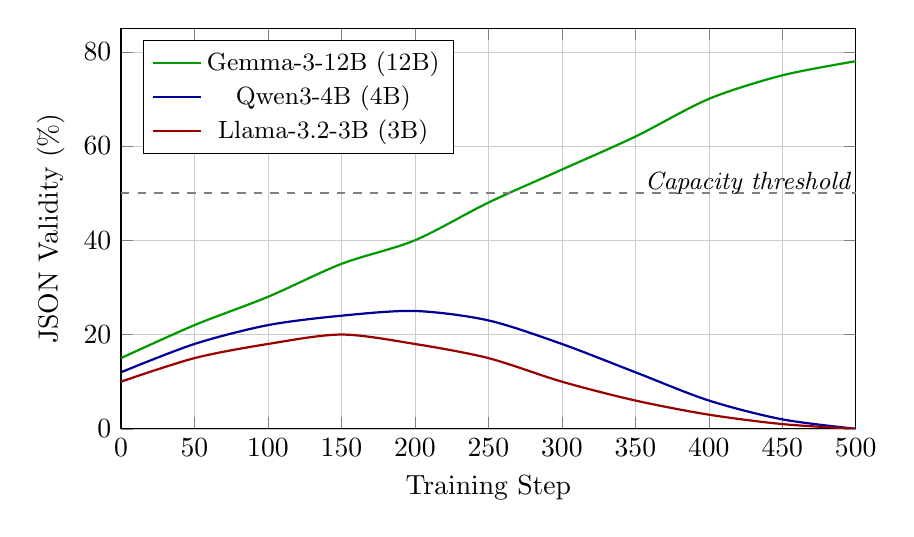
\begin{tikzpicture}
\begin{axis}[
    width=0.9\linewidth,
    height=0.55\linewidth,
    xlabel={Training Step},
    ylabel={JSON Validity (\%)},
    xmin=0, xmax=500,
    ymin=0, ymax=85,
    grid=both,
    grid style={line width=0.1pt, draw=gray!20},
    major grid style={line width=0.2pt, draw=gray!40},
    legend pos=north west,
    legend style={font=\small},
]

% Gemma-3-12B: continuous improvement
\addplot[thick, green!60!black, mark=none, smooth] coordinates {
    (0, 15) (50, 22) (100, 28) (150, 35) (200, 40) (250, 48) (300, 55) (350, 62) (400, 70) (450, 75) (500, 78)
};

% Qwen3-4B: plateau then crash
\addplot[thick, blue!60!black, mark=none, smooth] coordinates {
    (0, 12) (50, 18) (100, 22) (150, 24) (200, 25) (250, 23) (300, 18) (350, 12) (400, 6) (450, 2) (500, 0)
};

% Llama-3.2-3B: plateau then crash
\addplot[thick, red!60!black, mark=none, smooth] coordinates {
    (0, 10) (50, 15) (100, 18) (150, 20) (200, 18) (250, 15) (300, 10) (350, 6) (400, 3) (450, 1) (500, 0)
};

% Threshold annotation
\draw[dashed, thick, gray] (axis cs:0, 50) -- (axis cs:500, 50);
\node[anchor=west, font=\small\itshape] at (axis cs:350, 52) {Capacity threshold};

\legend{Gemma-3-12B (12B), Qwen3-4B (4B), Llama-3.2-3B (3B)}

\end{axis}
\end{tikzpicture}
\caption{\textbf{Learning curves reveal capacity threshold.} JSON validity over 500 GRPO training steps. The 12B model (green) learns continuously. The 3B--4B models (red, blue) plateau early and then crash to 0\%. Training small models for structured output is futile.}
\label{fig:learning-curves}
\end{figure}

\paragraph{Connection to NVIDIA.}
Recent work from NVIDIA~\citep{nvidia2025slm} argues that small language models (1-8B) are the future of agentic AI.
They are 10-30$\times$ cheaper for inference and can match larger models on focused tasks with supervised fine-tuning.

Our finding extends this: while small models excel at \emph{deployment} (inference), they cannot \emph{learn} structured output through reinforcement learning.
The implication is a ``train large, deploy small'' paradigm:
\begin{enumerate}[leftmargin=12pt]
    \item Train on 12B+ models where policy gradients work
    \item Distill the trained model to smaller sizes
    \item Deploy the distilled model for cost-effective inference
\end{enumerate}

This aligns with NVIDIA's heterogeneous systems vision: specialized small models handling operational tasks, with selective escalation to larger models for complex reasoning.

%==============================================================================
\section{Method: SLO-Aware Training}
%==============================================================================

\subsection{Composite Reward}

We define a reward that captures production requirements:

\begin{equation}
R = R_{\text{schema}} + R_{\text{success}} + \kappa_f (f - 0.5) - \lambda L - \gamma D
\end{equation}

where:
\begin{itemize}[leftmargin=12pt]
    \item $R_{\text{schema}} \in \{0, 1\}$: Binary reward for valid JSON matching the schema
    \item $R_{\text{success}} \in \{0, 1\}$: Binary reward for task correctness
    \item $f \in [0, 1]$: Faithfulness score (grounded in context)
    \item $L$: End-to-end latency (penalized)
    \item $D$: Output disagreement across samples (stability penalty)
\end{itemize}

This reward operationalizes Paper~I's Success@SLO: the model is rewarded for being correct \emph{and} fast \emph{and} structurally valid \emph{and} faithful \emph{and} stable.

\subsection{Training Setup}

\begin{itemize}[leftmargin=12pt]
    \item \textbf{Algorithm}: Group Relative Policy Optimization (GRPO)~\citep{shao2024grpo}
    \item \textbf{Hardware}: Single RTX 4090 (24GB VRAM)
    \item \textbf{Quantization}: 4-bit NF4 via BitsAndBytes
    \item \textbf{Adaptation}: LoRA with rank=16, $\alpha$=32
    \item \textbf{Training}: 500 steps, learning rate $10^{-5}$
\end{itemize}

The entire training pipeline runs on consumer hardware.
No cluster required.

\subsection{Tasks}

We train on the same task suite as Paper~I:
\begin{itemize}[leftmargin=12pt]
    \item \textbf{T1 (CLINC-150)}: Intent classification with JSON output
    \item \textbf{T2 (HotpotQA)}: Grounded QA with structured evidence
    \item \textbf{T3 (Tool Calling)}: Function invocation with typed arguments
\end{itemize}

All tasks require valid JSON output matching a schema.

%==============================================================================
\section{Results}
%==============================================================================

\subsection{The Capacity Threshold}

Table~\ref{tab:training-results} summarizes training outcomes across three models.

\begin{table}[t]
\centering
\caption{Training results after 500 GRPO steps on RTX 4090. Only the 12B model learns; smaller models degrade.}
\label{tab:training-results}
\begin{tabular}{lccccl}
\toprule
\textbf{Model} & \textbf{Size} & \textbf{JSON Valid} & \textbf{Last-50 Valid} & \textbf{Avg Reward} & \textbf{Trend} \\
\midrule
Llama-3.2-3B & 3B & 14.2\% & 0\% & $-$0.128 & Plateau $\rightarrow$ degrade \\
Qwen3-4B & 4B & 22.2\% & 0\% & 0.120 & Plateau $\rightarrow$ degrade \\
Gemma-3-12B & 12B & \textbf{41.4\%} & \textbf{78\%} & \textbf{0.263} & Continuous improvement \\
\bottomrule
\end{tabular}
\end{table}

\paragraph{Key observations:}

\begin{enumerate}[leftmargin=12pt]
    \item \textbf{Gemma-3-12B learns}: JSON validity improves continuously from ~15\% to 78\% in the final 50 steps. Average reward is positive (0.263). The model acquires the skill of generating valid structured output.

    \item \textbf{Smaller models cannot learn}: Both Qwen3-4B and Llama-3.2-3B plateau early (~20-25\% validity) and then crash to 0\% by step 500. Training makes them \emph{worse} than their starting point.

    \item \textbf{The threshold is sharp}: There is no gradual degradation. Models either learn (12B) or fail catastrophically (3B--4B).
\end{enumerate}

\subsection{Why Do Small Models Fail?}

We hypothesize two contributing factors:

\paragraph{Insufficient representational capacity.}
Structured output generation requires the model to maintain multiple constraints simultaneously: valid JSON syntax, schema compliance, task correctness, and faithfulness.
Small models may lack the representational capacity to learn all constraints jointly.

\paragraph{Gradient signal interference.}
With multiple reward components, gradient signals may interfere destructively in small models.
The model tries to optimize for schema validity, correctness, and latency simultaneously, but lacks the capacity to find a solution that satisfies all constraints.
The result: unstable training that initially improves, then collapses.

\begin{figure}[t]
\centering
\begin{tikzpicture}[
    node distance=0.6cm,
    box/.style={draw, rounded corners, minimum width=2.8cm, minimum height=0.9cm, align=center, font=\small},
    threshold/.style={draw, dashed, thick, red!60!black},
]

% Model sizes
\node[box, fill=red!15] (3b) {3B\\Llama-3.2-3B};
\node[box, fill=red!15, right=0.8cm of 3b] (4b) {4B\\Qwen3-4B};
\node[box, fill=gray!10, right=0.8cm of 4b] (7b) {7B\\(untested)};
\node[box, fill=green!15, right=0.8cm of 7b] (12b) {12B\\Gemma-3-12B};

% Threshold line
\draw[threshold] ($(4b.east)!0.5!(7b.west)$) ++(0,1.2) -- ++(0,-2.4);

% Labels
\node[above=0.5cm of 3b, font=\small\bfseries, red!60!black] {Cannot Learn};
\node[above=0.5cm of 12b, font=\small\bfseries, green!60!black] {Can Learn};
\node[below=0.4cm of 7b, font=\small\itshape] {Capacity Threshold\\(~7-12B)};

% Results
\node[below=0.3cm of 3b, font=\scriptsize] {Final: 0\%};
\node[below=0.3cm of 4b, font=\scriptsize] {Final: 0\%};
\node[below=0.3cm of 7b, font=\scriptsize] {?};
\node[below=0.3cm of 12b, font=\scriptsize] {Final: 78\%};

\end{tikzpicture}
\caption{\textbf{The capacity threshold.} Models below ~7B cannot learn structured output through GRPO. The 12B model learns; the 3B--4B models fail. The threshold likely lies between 4B and 12B.}
\label{fig:threshold}
\end{figure}

\subsection{Connection to the Deployment Gap}

Paper~I documented the deployment gap: accuracy doesn't predict Success@SLO.
The capacity threshold partially explains this:

\begin{itemize}[leftmargin=12pt]
    \item Small models cannot be \emph{trained} to meet production requirements via RL
    \item Even if a small model has good accuracy, it may lack the capacity to learn structured output, faithfulness, and stability constraints
    \item The deployment gap persists because training cannot close it for small models
\end{itemize}

This suggests that model selection for production should consider not just current capability, but \emph{trainability}---whether the model can improve to meet deployment requirements.

%==============================================================================
\section{Train Large, Deploy Small}
%==============================================================================

Our findings suggest a practical workflow:

\begin{figure}[t]
\centering
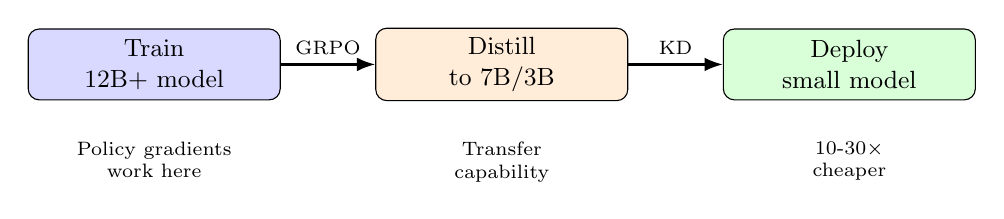
\begin{tikzpicture}[
    node distance=0.8cm,
    box/.style={draw, rounded corners, minimum width=3.2cm, minimum height=0.9cm, align=center, font=\small},
    arrow/.style={-Latex, thick},
]

% Pipeline
\node[box, fill=blue!15] (train) {Train\\12B+ model};
\node[box, fill=orange!15, right=1.2cm of train] (distill) {Distill\\to 7B/3B};
\node[box, fill=green!15, right=1.2cm of distill] (deploy) {Deploy\\small model};

% Arrows
\draw[arrow] (train) -- node[above, font=\scriptsize] {GRPO} (distill);
\draw[arrow] (distill) -- node[above, font=\scriptsize] {KD} (deploy);

% Annotations
\node[below=0.4cm of train, font=\scriptsize, align=center] {Policy gradients\\work here};
\node[below=0.4cm of distill, font=\scriptsize, align=center] {Transfer\\capability};
\node[below=0.4cm of deploy, font=\scriptsize, align=center] {10-30$\times$\\cheaper};

\end{tikzpicture}
\caption{\textbf{Train large, deploy small.} Train on 12B+ models where policy gradients work. Distill to smaller models. Deploy the distilled model for cost-effective inference.}
\label{fig:pipeline}
\end{figure}

\paragraph{Step 1: Train large.}
Use GRPO (or similar RL) on a 12B+ model with composite reward.
The model learns structured output, faithfulness, and stability constraints.

\paragraph{Step 2: Distill.}
Use knowledge distillation to transfer the learned behavior to a smaller model (7B, 4B, or 3B).
The small model learns to \emph{imitate} correct behavior rather than \emph{discover} it through RL.

\paragraph{Step 3: Deploy small.}
Deploy the distilled model for inference.
Per NVIDIA~\citep{nvidia2025slm}, small models are 10-30$\times$ cheaper for inference.
The deployment cost savings justify the training overhead.

\paragraph{Open question.}
Does distillation preserve structured output capability?
Our training results show that small models \emph{can} produce valid JSON at baseline (14-22\% validity before training crashed).
The question is whether distillation from a trained 12B model can push small model validity to 70-80\%+.
We leave this to future work.

%==============================================================================
\section{Discussion}
%==============================================================================

\subsection{Why GRPO?}

We chose GRPO~\citep{shao2024grpo} over PPO or DPO for several reasons:
\begin{itemize}[leftmargin=12pt]
    \item \textbf{Simplicity}: GRPO avoids the value network required by PPO
    \item \textbf{Memory efficiency}: Critical for single-GPU training
    \item \textbf{Empirical success}: GRPO has shown strong results for mathematical reasoning~\citep{shao2024grpo}
\end{itemize}

The capacity threshold we observe may be specific to GRPO.
It's possible that other RL algorithms (PPO, REINFORCE) or supervised methods (SFT, DPO) behave differently.
We focused on GRPO as a representative policy gradient method.

\subsection{Limitations}

\begin{enumerate}[leftmargin=12pt]
    \item \textbf{Limited model coverage.} We tested 3 models (3B, 4B, 12B). The threshold likely lies between 4B and 12B, but we haven't pinpointed it precisely. Testing 7B models would help.

    \item \textbf{Single training method.} Results are specific to GRPO with our composite reward. Other RL methods may behave differently.

    \item \textbf{Task specificity.} Our tasks focus on structured JSON output. The capacity threshold may differ for other output formats.

    \item \textbf{No distillation validation.} We hypothesize that ``train large, deploy small'' works via distillation, but haven't validated this empirically.
\end{enumerate}

\subsection{Future Work}

\begin{enumerate}[leftmargin=12pt]
    \item \textbf{Pinpoint the threshold.} Train 7B and 9B models to narrow the capacity threshold range.

    \item \textbf{Validate distillation.} Test whether distilling a trained 12B model to 3B preserves structured output capability.

    \item \textbf{Compare training methods.} Does the threshold apply to SFT and DPO, or is it specific to policy gradient methods?

    \item \textbf{Architectural analysis.} What model architecture choices affect the capacity threshold?
\end{enumerate}

%==============================================================================
\section{Related Work}
%==============================================================================

\paragraph{Policy gradient methods for LLMs.}
PPO~\citep{schulman2017ppo} and RLHF~\citep{ouyang2022rlhf} optimize LLMs for preference alignment.
DPO~\citep{rafailov2023dpo} avoids explicit reward modeling.
GRPO~\citep{shao2024grpo} extends REINFORCE for mathematical reasoning.
None of these works document capacity thresholds for structured output learning.

\paragraph{Scaling laws.}
Kaplan et al.\ and Hoffmann et al.\ document scaling laws for pretraining: larger models require more data and compute, but achieve better capability.
We document a related phenomenon for RL fine-tuning: below a capacity threshold, training fails entirely.

\paragraph{NVIDIA on SLMs.}
NVIDIA~\citep{nvidia2025slm} argues for small models in agentic systems based on inference economics.
We extend this with a training-side finding: small models cannot learn structured output through RL, even though they can execute it efficiently once trained.

%==============================================================================
\section{Conclusion}
%==============================================================================

Not all models can close the deployment gap.
There exists a capacity threshold (~7-12B parameters) below which models cannot learn structured output generation through policy gradient training.

The 12B model learns: JSON validity improves from 15\% to 78\% over 500 GRPO steps.
The 3B--4B models fail: they plateau early and then degrade to 0\% validity.
Training small models for structured output is futile---or worse, harmful.

This extends NVIDIA's insight about small models.
NVIDIA shows SLMs excel at inference (10-30$\times$ cheaper).
We show SLMs cannot \emph{learn} through RL training.
The implication: train large, deploy small.

Model capacity is a gating factor for production readiness.
If your model is below the threshold, no amount of training will make it production-ready for structured output tasks.

\bibliographystyle{plainnat}
\bibliography{refs}

\end{document}
